
\chapter{Gunslinger Girl}

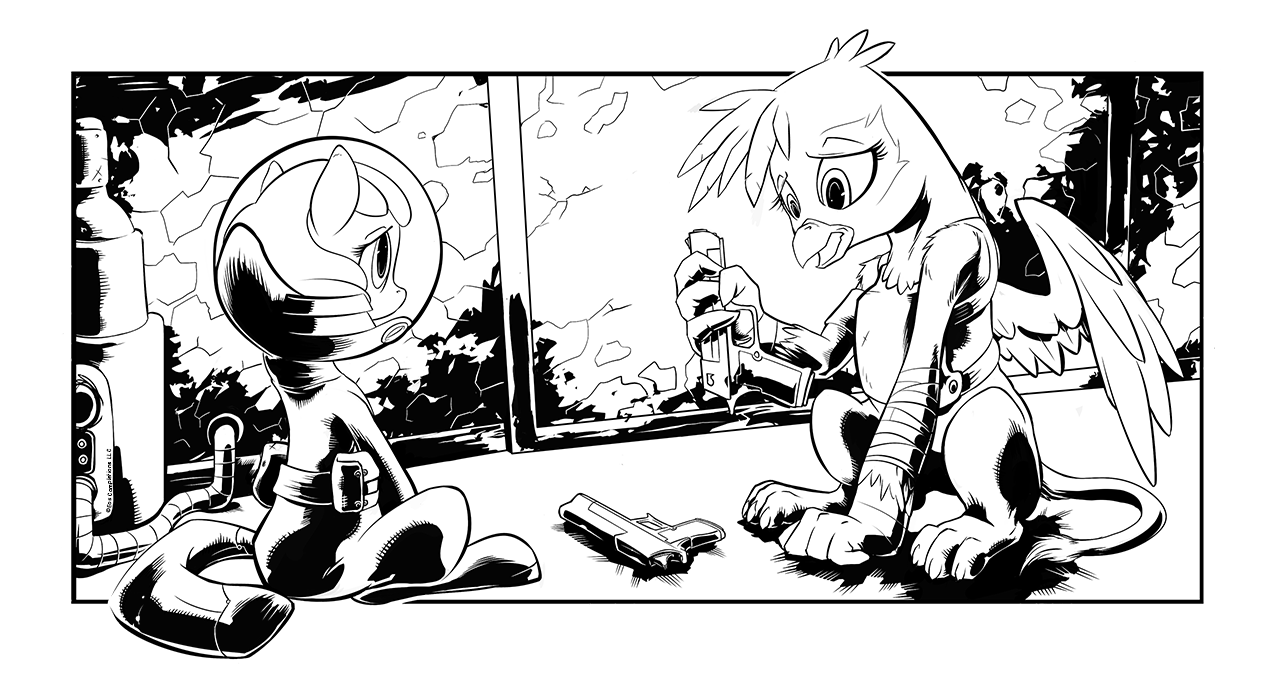
\includegraphics[width=0.9\linewidth]{image06.png}

\begin{intro}
Well, now, uh, Lancelot, Galahad, and I, wait until nightfall, 

and then leap out of the rabbit, taking the French by surprise---

not only by surprise, but totally unarmed!
\end{intro}


\rtpr{``Good evening my beautiful herd! This is Lonesome Pony, and you're listening to Radio 52, the frequency that gives you all the essentials about the Big 52 and nothing else!''}

The evocative tinkling of dueling banjos filled a brief intermission.

\rtpr{``Let's get to work. Have you ever wondered what the sun looks like? Ask the White Apples! Last night, a gigantic ball of light exploded ten kilometers east of Salt Cube City, leaving thunder and devastation in its wake. Luckily enough, along said wake there were mostly radigators and abandoned shacks, but the light could be clearly seen even from Tunnel Town, the Badlands, and the Redtrotters territory. If you think this is crazy, I must warn you that it was just the last act of a night of follies! First we had the launch of a balloon full of ghouls; yes, the very same ghouls that threatened the caravans in the area! The take-off was accompanied by a light and magic show offered by a certain Puppysmiles. Weird name, isn't it? This is not the first time I've had something to say about this gal. Good old L.P. asked some more questions here and there, and guess what he discovered? Yes, she's the same filly from the Carnival!''}

A trumpet erupted in triumphant fanfare.

\rtpr{``So, Lonesome Pony, where's the interesting part? Here it is for all those grumpy `too long didn't listen' busy ponies on the road: no more feral attacks between the Badlands and the Cube!''}

There was the sound of a reloading lever action rifle followed by pair of gunshots and a very manly voice saying, ``\rtpr{Hasta la vista, filly.}''

\rtpr{``Oh yes, I love this one! Two tribes get their problems solved by a foal stuck in a radsuit! Now, I don't need to be a shaman to know that she's heading south, so, what's next? Is she going to reopen the Tunnel? Well kid, if you happen to stop by trade station Badlands on the Marshes detour, pay a visit to your number one fan! We'll get to know the filly inside the helmet! Till then, have some music from the best radio station you can find along the Route.''}

\begin{music}
		``Here's a pony there's a pony
	
		and another little pony
	
		funny pony party pony
	
		pony pony sprite\dots''
\end{music}

\horizonline

\englishdaytimeplace{5}{16:45 P.M.}{165Th Brigade field Headquarters, Salt Marshes}

``Stop that damn music, I can't hear if he's still outside!'' the young griffon snapped at Puppy while shooting her an exasperated glare.

``B-but it's funny! You're a grumpy chicken!'' Puppy frowned and went back to hugging her Pinkie Pie plushie. ``Don't worry, Silky Tail, she's not mad. She's just a bit tired.''

Henrietta the Griffon walked over to Puppysmiles and grabbed the filly's helmet so that she could look her in the eye. ``For the last time, I am NOT a chicken! There's a freaking manticore out there that's pinned us inside this place, and you are doing your most to drive me crazy!'' Her voice broke in a shrill screech. ``I hope that my father arrives soon.'' She sighed. ``Maybe with his help we'll be out of here, and I'll never ever need to see your stupid face again!''

``I'm not stoopid! You're a meanie cat and I don't want to be your friend anymore!''

{\mten ``Warning. Hostile griffon at three meters. Threat level: High.''}

``Aw, shut up, Mister Voice.'' Puppy turned her back on Henrietta in a theatrical display of sulking.

``Shut up mister who? Who are you talking with now?'' Henrietta raised an eyebrow. ``You have a radio transmitter in that thing?'' With a jump, Henrietta was on Puppysmiles, trying to take off her helmet. ``We can call for help! Call my father on 90.08! Codename Blaze!''

Puppy was taken by surprise. ``Hey wait! I have to ask Mister Voice! He lives inside the suit and works all the weird things!'' She tried waving a hoof to shoo Henrietta away, but she was already stepping aside.

``Wait. Mister Voice? That suit talks?''

``Sure it does! This is the best space suit ever! And it is also super smart!'' Puppy smiled proudly.

``Yeah,'' Henrietta snickered. ``I bet it's smarter than you.''

``Sure! Smarter than---'' Her smile became a frown. ``Hey! That's not very nice!''

Henrietta was already laughing. ``I can't believe you fell for that! You're hilarious! Dumber than a banana pajama!'' Henrietta smiled and gave Puppy a bump with her paw.

``H-hey, stop that! You meany-mean chicken! If your dad wasn't that hurt, I'd have already given you a lesson!''

Henrietta froze in place, staring at Puppy. ``My father what? What do you know about my father?'' Hope and fear were mixing on her face in a concoction that made even Puppysmiles aware that her next words needed to be used very, very wisely.

``Uh, last time I saw him he was dead. Maybe he got better?'' She smiled, helplessly lost in childish naivete.

``M-my father\dots died? How do you know that? Where have you seen him? This---this can't be, he's the best around; he can't be dead! You're wrong, this can't be true! Tell me that this isn't true!'' She drew her white pistol and aimed it at Puppy, the yellow line along the barrel pointed directly at her nose. ``Tell me that you're wrong!''

Puppy met Henrietta's wild gaze. She could be a bit slow, but there was no lie in those gleaming pink eyes, just the absolute innocence of a child. ``I\dots I don't know. He wanted me to say to you that he really, really wanted to be here and he was sorry. I ran here in a super hurry to find you because he was really sad and I felt bad for him and I lost my mom too---''

\emph{``Enough!''} Henrietta batted Puppy's helmet with a claw, knocking her against a wall, before curling up on herself, trying to hide her face from the harsh reality. ``This isn't true\dots My dad is the best hired gun ever! He's okay, I'm sure he's heading here right now! Fuck, I\dots I\dots'' A soft metallic sound made the girl open her eyes.

Puppy stood in front of Henrietta. She didn't say anything, but took the black gun with the red line along the barrel from her saddlebag and left it next to Henrietta before going back into a corner of the small room.

``Black Rose.'' She stared at the gun in surprise as she came to realize what she already knew. ``Oh no\dots No, please! This can't be true\dots'' Again, she looked at Puppy. ``Please, tell me this isn't real. Tell me this is a bad dream!''

Puppy frowned and looked down. ``I don't know. If this is a bad dream, then I'll wake up and find my mom waiting for me, so\dots I also hope that this is all just a really long bad dream.'' She sighed. ``But I don't think it is.''

``Fuck\dots'' Henrietta took the gun in a claw, looking at it and extracting her own .45 Auto pistol. They were identical in every detail except for the color. ``How did it happen? Why were you there?'' \emph{Keep flying Henrietta, don't snap now. You learned from the best. You can do better. You \emph{must} be better.}

``There were four chickens fly---''

``STOP CALLING US CHICKENS! We are griffons, and we're better than you filthy ponies! Call me, or another griffon a chicken again and I'll make sure that it will be the last time! Capeesh?'' She held Puppy by the neck, keeping her lifted off the ground while she pressed a gun into Puppy's chest with her other claw.

Puppy's eyes were filled with fear. She tried to break free, but after a quite useless struggle, she simply gave up and began to cry. ``I-I'm sorry, Miss Griffon! I'll behave! Please stop! Please!''

Henrietta nodded and put her down. ``Way better. Now, there were four griffons. Where and when?'' That burst of anger somehow washed away the first shock, allowing Henrietta to focus more clearly on the situation before her.

Puppysmiles talked fast, trying her best not to disappoint the scary griffon again. ``It was earlier. I was going down the road with a friend and they were in the sky. At the beginning it seemed that they were doing a pretty show, but then a lot of them got hurt and they fell from the sky and then they were all dead. I spoke with the last one before he was dead and he told me to come here and give you that black thing and to say to you that he was sorry and that he wanted to go south and then I poked him to make him open his eyes, but he kept sleeping but I tried really hard to wake him! Please don't be mad at me, I really really wanted to make him get better, but he didn't move and then Mister Voice told me that he was dead and\dots and\dots'' She stepped back, gasping for air and putting both hooves above her head in an attempt to hide herself. ``Please stop bullying me! I didn't want to be mean I just wanted to help! I'm sorry!''

\emph{Fuck, she's just a kid.} Henrietta hesitated as her anger began to fade. That foal probably didn't even mean chicken as an insult. Nonetheless someone had to teach her something before she got into real trouble.

``And guess who that someone is,'' muttered Henrietta. Sighing, she patted Puppy's helmet. ``It's cool, really. Call me Henrietta or Henri, okay? You just lack some, uh, style, but don't worry, you'll learn. Now let's find a way out of here.''

``But, but you're mad at me!'' Puppy was still hiding her head behind the hooves.

``No, I'm not mad. Now be a good pony and stand up, okay?''

``But I called you a chicken, and I told you that you were mean.''

``Just don't do that again, okay? I scolded you and now we are even. All right?''

``So, so we can still be friends?'' Puppy tried hopefully.

She sighed. ``Yes, we can still be friends. Now please be quiet while I think of a plan.''

Yes, sure, it was easy to say, maybe a little harder to carry out, but even those simple words were enough to renew Puppy's happy-go-lucky mood. Puppy nodded and sat next to the stairs, while Henrietta took a look outside. The predator had to be hiding somewhere, probably waiting for them to venture out in the open.

``Not good. If only I had something better than my guns. I could hope for a lucky shot, but if I miss\dots'' She looked back at Puppy. ``Hey, you don't happen to have a large caliber gun or some high explosives, do you?''

``I have a rock! It's super rocky!'' Puppy proudly showed \emph{The Rock Of Destiny} to Henrietta.

That made Henri snicker. ``Oh yes, exactly what we need, a rock. Sorry kid, but I don't think that I'll let a stupid rock decide my fate.''

Puppy tilted her head, then looked a bit confused at her favored weapon. ``I don't think that you're dumb, Rock, but now it's better that you go back sleeping.''

``Please! I'm trying to put a plan together here. Stop kissing goodbye to everything you stash in your saddlebags and do something useful like---'' Henrietta hesitated. ``Like, ah, on second thought, just go back and play with Twinkle Sail.''

``Silky Tail!''

``Yeah, that one. Have fun.''

``Okie dokie! The tea will be served in five minutes!'' Puppy sat down on the stairs, taking the stuffed Pinkie Pie from her bag.

``Yes, whatever. Now\dots'' She lowered her voice to a mumble. ``There's no decent cover, and I'm not sure that I can outrun that thing for more than a couple of minutes. We have to face it, but we lack the firepower.'' Henrietta sighed in distress. ``This is ridiculous. Those tanks are full of high explosive ammunition, and we are stuck here with three .45s and a uh, rock.''

In the meantime Puppy sat her doll on a large Flack 8.8 projectile while using another one as a teapot to serve tea. ``Hey, do you want six or eight sugar cubes in your cup? Ah, do you have a cup?''

``No thanks. I think I have a plan,'' she said without even bothering to turn back to Puppy. ``I'll run outside and try to get the manticore's attention. After the manticore starts chasing me you'll sprint to the nearest tank and get inside. You have to be fast because I can't distract that thing for very long. When you're in the tank you have to look for HE ammo. They're big and shiny, like a big can with a pointy head. They should have a red band so they are easy to identify. All right?''

``Uh, yes.'' Puppy looked for a moment at her ``teapot'', then shrugged and put it away. ``You just keep an eye on Silky Tail, okay?''

``I don't think that your doll is going anywhere while we're out. Just go inside the tank, grab the big can with the red line and run back here. When you're done I'll explain to you the second part of the plan.'' Henrietta crouched, readying herself for a jumping start. She needed all the speed she had.

``But she'll be afraid!'' Henri turned around and scowled. That filly was a constant source of idiocy and distraction.

``Puppy, Twinkle Sail is just a doll! It can't be afraid!'' Henrietta walked over to the stuffed Pinkie Pie/Silky Tail, grabbing it and waving it around in front of Puppy. ``See? She's smiling, so she's okay! Maybe when we get back she will throw us a\dots HE Flack 8.8?'' Her eyes focused on the object being used as a chair for Puppy's toy. ``Pardon me. Where did you find this?''

Puppy smiled. ``Soft Air gave me Silky Tail in the Glow.'' 

``No, I mean this one. The 'chair'.''

``Oh that. It was inside a broken super huge metal cart. It's shiny and clean, and I've got plenty of them.'' From the expression on her face Puppy felt that she had to say something more. ``Do you want one?''

Henrietta's left eye went twitchy twitch. ``Okay, great. Part one done. Now for part two.''

``What? But we didn't even---''

``No, just no. I said part two, let's never speak of part one again.'' Her self control was considerably improving. ``Listen carefully. I'm trying to lure Mister Big Bad here into the tower entrance. When the manticore pokes his head in you have to throw the shell into his mouth, and then I'll shoot it. The head goes boom and no more bullies, got it?''

Puppy frowned. ``So, I throw the teapot inside the jaws and the movie ends?''

``The what? Yeah, sure, throw that thing in the manticore's mouth and I'll do everything else. Now get ready and don't be scared, okay?''

``Okie dokie!'' She hugged the shell and hid herself behind the wall while Henrietta cautiously stepped out of the building with her wings outstretched.

Not even a minute later, the sound of gunshots came from outside, followed by the voice of a griffon who was teasing the manticore with a lot of words that Puppy never heard before. She was super double curious about what was going on outside, but she had been told to stay put and wait. Now this was a dilemma. If Henrietta found her out of place, she was going to be really mad, and that girl was really scary when she was mad! On the other hoof, Puppy was sure that there was something totally cool going on just a few steps away from her.

``Maybe just a little peek.'' Outside, it rained lead as beastly roars thundered in the storm of the battle. ``Just one peek won't hurt, right?'' She slowly crawled next to the door, hugging her HE shell and trying to look outside. ``Sneaky sneaky\dots''

``Aw, I can't see a thing! This isn't fair at all---''

Suddenly a blurry silhouette came speeding through the door, rushing to the opposite side of the room and yelling, ``NOW!''

``Now what?'' asked Puppy a little surprised.

\emph{ROAR!}

Snarling and scraping at the concrete, the manticore appeared at the door, trying to get inside, but being held out by its size. Puppy found herself looking into the snapping jaws of a fell beast just a few inches away from her helmet and yelped, backpedaling.

``Puppy, what are you doing? Throw that thing now and dive for cover!'' The urgency in Henrietta's voice danced with the panic in her eyes. ``Move that cutie mark!''

Puppy nodded and tried launching the shell. The high explosive round traced a straight trajectory through the air while Puppy jumped as far away as she could. When the explosive ammunition hit the ground right below the beast's head the griffon opened fire.

\emph{BLAM! BLAM! BLAM!}

Three shots, three hits, three bounces. ``Fuck! Its case is too thick; I can't penetrate it!'' She swore and emptied both pistols against that stupid explosive shell to no avail.

``It's not working!'' Henrietta put away one of her guns and took a third pistol. This one was red with a white line along the barrel, but in everything else it was identical to the other two she had. Unloading the gun directly in the manticore's muzzle, she succeeded in making the monster slow down his assault for a moment.

``I think he's trying to make the door larger.'' Puppy stepped back another couple of meters but now she seemed a lot less scared. She tapped her helmet as if she was pondering the situation. ``He's good.''

The beast was looking at Henrietta with bloodlust in his eyes. It was clear enough that he wasn't going to lurk any longer, even if that meant tearing apart the whole tower. The real issue was that the manticore was actually tearing the building apart. Maybe not very fast, but he was getting there.

``Don't just stand there! Come here!'' Henrietta reloaded her pistols. ``We can still make that thing go boom if only I can hit the detonator. You just stay low, I'll try something!''

``What's a dee-tuna thor?''

Henrietta launched herself toward the manticore, ignoring Puppy's question. With a leap she arrived just a couple of slashes out of the beast's reach and pointed both guns at the shell. ``Say goodbye, Josè---'' It was already too late. She noticed that the predator had his head reclined and his back arched. Henrietta was half feline, so she knew just how much a manticore could stretch. She should have known better than to get so close. The cat had just fallen into the lion's jaws, and he didn't even give her time to swear.

In an instant, the manticore stretched out and struck the griffon with a claw, hitting her in the shoulder and grabbing her with his mighty talons. Henrietta shrieked in pain and instinctively but uselessly pecked and bit at the monster's paw.

Puppysmiles screamed in terror, too. She tried to back away further, but her rump was already pressed against the wall. This manticore was terrible, but, even worse, he was hurting Henri.

For a moment Puppy saw not a manticore in front of her, but a pink metal face with blinking blue eyes.

\emph{Please ‒giggle‒ make this ‒giggle‒ end.}


Puppy's eyes flared with pink flames as she raised her hoof. ``Rock!'' As soon as \emph{The Rock Of Destiny} was in her hoof she launched herself against the beast. ``Let her go! Let her go NOW!''

The manticore immediately spotted the yellow critter assaulting him and instinctively turned his head and closed his jaws on her, tossing his old prey aside. The fangs of the monster closed on her, crushing her with a dry, crunchy sound. Henrietta fought to stay conscious while she staggered across the room trying to reach the stairs. In the meantime the manticore let out a triumphant roar that sealed once and for all Puppy's fate.

``No, no, it's too late\dots Save yourself gal. Don't turn back\dots'' Weakly, she climbed a couple of steps, but the pain was driving her crazy. The manticore behind her was howling in a bloody, ponycidal rage, probably tearing apart and dismembering every limb of that poor corpse. Henrietta took a healing potion and swallowed it all in a single gulp before falling face down, her sight now beginning to fail. Henri tried to turn over to see what was going on and why that atrocious beast kept roaring and howling, but all she could see was a thick pinkish smoke and nothing else. Then the griffon lost her battle against the staggering pain and fainted.

Now please, let's have a moment of silence for the truly unfortunate manticore.

\dots

And this is why rule number one says no biting. Ever. The meat might be spoiled.


\horizonline

\englishdaytimeplace{6}{00:45 A.M.}{165Th Brigade field Headquarters, Salt Marshes}

{\mten ``System successfully rebooted. All functions restored. Diagnostic system is online. Subject 001: Puppysmiles. Female earth pony. Subject deceased, condition stable. All clear.''}

Puppy lazily opened her eyes and yawned. ``But it's still dark outside\dots'' She had the unpleasant sensation of something heavy laying on her back. ``What happened? Where's the chicken? And the big meany kitty cat?''

{\mten ``Analyzing: hostile detected. six meters east. Henrietta. Threat level: negligible.'' A single red dot was blinking on the compass.}

``Silly Voice, Henri is not an enemy!'' The dot turned pink. ``Okie dokie, let's go to---hey!'' She moved her hooves, but this didn't make her go anywhere. Puppy looked down to see that she was hanging from some sort of gray perch. It took more than a couple of tries to break free from the skull of the manticore. The skeleton of the beast had turned the same color as the wall, and seemed to be partially stuck inside of it. It was as if the animal and the wall had melded together. The large head of the beast was open in an eternal roar while his wings stretched out, desperately trying to break free from the deadly cloud that had consumed him.

Puppysmiles trotted over to Henrietta, but the griffon was lying on the stairs, giving no signs of life. ``Mister Voice, is she, you know, uh, dead?''

{\mten ``Analyzing: negative. The subject is unconscious.''}

``Oh. This means that she will be okay?''

{\mten ``Affirmative. The subject is recovering.''}

``Okie dokie.'' That was enough for Puppy. She smiled and kissed Henrietta goodbye through her helmet. ``I'm sorry, but I still have to go, Chicken Girl. My mom is somewhere on the other end of this arrow.''

Puppy trotted some meters away, but then stopped and frowned. Somehow she felt that just kissing goodbye this time wasn't enough. She went back to Henrietta, took the Pinkie Pie doll from her saddlebags, and put it under one of Henri's talons.

``Here, Silky Tail. Look after Henrietta and don't let anything bad happen to her.'' Now it was really okay. Puppy trotted outside and retrieved her scooter.

``Hey, can I has some music?''

\begin{music}
		In the jungle, the mighty jungle,
	
		the lion sleeps tonight!
	
		In the jungle, the quiet jungle,
	
		the lion sleeps tonight\dots
\end{music}

\horizonline

\englishdaytimeplace{6}{10:00 A.M.}{Griffon's Fall, Salt Marshes}

Digging in a marsh without a shovel was already torture by itself, but digging your father's grave in this muddy terrain with your bare claws was\dots No. Just no.

Tears dropped from her beak as she swallowed back the pain. Every time she tried deepening the hole in the dirt it was filled again with murky water, but she continued digging in silence. He could never bear her crying, and he was the most hardened badass mercenary ever. And now he was dead, killed by Talons.

Henrietta dragged the dead body to the shallow hole and pushed him inside. The corpse settled into the mud with a gurgle. She watched the blood-stained feathers sinking in the pool as she tried her best to fight back the tears. Fuck\dots He wouldn't even sink in completely.

``Not fair, man, leaving me alone like this. What am I going to do now?'' Henrietta sighed. She tried being mad at him, if only to have some weapon against her grief, but it was so hard. He was gone, so what now? ``Why you\dots''

Fuck.

Just fuck.

She began filling the grave again with mud and all the stones and asphalt chunks she could find nearby. With the last stone in place, Henrietta stared at where his beak had been visible just moments before. She took out the black gun and hesitated, then put it away again. Instead, she plucked three cerulean feathers from her right wing and planted them where she knew her father's chest would lie forever.

``Tell Mom I'll be fine, okay?''

Henrietta rubbed her eyes with one claw while she rummaged in her bag with the other, retrieving Silky Tail. She looked into the smiling blue eyes of the stuffed doll and tried to smile back. ``I'll be fine.''


\horizonline

\englishdaytimeplace{6}{11:30 A.M.}{Random encounter location, Salt Marshes}

``Hi! I'm Puppysmiles!''

One of the three slavers, a black earth pony, frowned. ``I think I heard that name before. Maybe we should just pass on this one.'' He looked at the other two ponies. They were all well armed, but over the last two days Lonesome Pony kept rambling on about a ghost infesting the northern branch of the Big 52.

``I'm not afraid of ghosts, Dripping Blood, but if a foal scares the shit out of you then just keep an eye on the other slaves.'' The leader of the slavers, a yellow unicorn, glared at his meager haul: a couple of stallions and a foaling mare. Way below the quota. ``Forty Nails, catch her.''

Puppysmiles was a bit uncertain. There were six dots on her compass, but half of them were pink and the other half were red. This had to be more weirdness by Mister Voice. One of the ponies marked with a red dot approached her cautiously and put a hoof on her back.

``Now come with us and don't resist, kid.''

``Okie dokie! Where are we going?'' Puppy smiled with enthusiasm.

Apparently her behavior was quite odd to these newcomers. The nearest pony, a green unicorn, looked over to his boss, who shrugged and encouraged him. ``See? Easy peasy. Put her in a collar and let's move.''

Forty Nails tried to open Puppy's Suit, but he wasn't exactly a Ministry of Peace technician. ``Hey boss, this fucking thing won't open!''

``Uh-uh. I can't take it off too. It's a super stuck helmet. I even tried hitting it but it just keeps repairing itself!'' At last somepony was helping Puppy with the space suit problem, but they didn't seem anywhere skilled enough. ``I think that there is some sort of button to press here and there but they don't work.''

``Shut up, retard.'' Forty was losing patience and decided to go medieval on the whole problem. ``It's clobbering time.'' He held up a hydraulic wrench and brought it down hard on Puppy's helmet, creating an intricate network of cracks that ran across its surface.

The yellow unicorn roared. ``Hey, if you break her head I'll break yours! A dead foal is worth nothing!'' The black slaver simply kept an eye on the other three slaves snickering at the scene.

Puppy stepped back, afraid. ``Hey, that's dangerous!''

{\mten ``Warning. Compass malfunctioning. Warning. Sensor system offline. Warning. Helmet integrity severely compromised. Repair system activated.''}

``Fucking Sun, that's a hard nut to break!'' The green unicorn raised his weapon again, only to see that the cracks in the helmet were already closing. ``What the fuck?'' He hesitated.

``Just tie her up with a rope and let's get going. We'll see to that once we're out of this shit hole.''

Puppy was told to behave, so she behaved while the pretty ponies put a noose around her neck. It was only when they tried dragging her with the other slaves that she began feeling something wrong in the air.

``Hey, I can't leave my ride there!'' She trotted toward her scooter, but the slaver holding the rope stopped her with a sudden jerk.

``Where do you think you're going?''

Puppy kept struggling. ``My scooter! Lemme go!''

Forty Nails snickered. ``Yeah, sure bitch.'' He pulled her close and looked into her eyes. ``You're a slave now. Forget your scooter and everything else. If you want to stay alive, stay put. Got it?''

``Uh, but I have to go there!'' Puppy pointed a hoof south. The green unicorn snorted and hit her on the flank with the butt of his hunting rifle.

``Shut up and open your ears or I'll rape you hard! Rebel ponies are bad commodities anyway.'' Forty turned to the slaver's leader. ``Hey boss, I'm teaching this one a little respect.''

``Don't mess her up or you'll be paying for her.'' The leader shrugged without even turning back.

Puppy frowned. ``I don't think that's a nice word\dots'' She seemed completely unfazed by the first beating, so the green slaver gave her a stronger blow.

``SHUT! UP!''

Puppy was sent flying, landing a few meters away. ``Hey! Somepony could get hurt!'' She got up on her hooves, giving no sign of pain and earning a worried look from Forty Nails.

``B-but what are you? Fuck off and stay down!'' The slaver aimed his rifle and shot two bullets into the foal.

\emph{BLAM! BLAM!}

Two hits, two holes in the filly's chest, and still no reaction. Forty's eyes widened in terror. In the meantime the leader turned on his minion.

``What the fuck are you doing you fucking son of a fucking drug addict! This is the last time you kill a slave!'' The yellow unicorn rammed into the green pony head on, sending him flying through the air.

``No! I'm not gonna die here!'' In a state of utter panic, Forty turned his rifle against his boss and emptied the magazine, blowing off one of the unicorn's legs before he could even realize what was going on. The slave leader fell to his knees, pulling out his assault rifle and spraying bullets all around. The black earth pony that had kept silent until now unsheathed a shotgun but was hit by the raging boss along with one of the slaves and Puppysmiles. The bullets pierced the foal's suit, leaving at least three different holes. It didn't seem to affect her very much.

``Stop quarreling! Please! Hey! I'm talking with you too!'' Puppy tried to restore some order, but this brawl seemed a bit beyond her capabilities. ``You are all bad ponies and you should feel bad! Mister Voice, do something!''

{\mten ``Repairs finished. Containment fully restored. Subject 001 Puppysmiles deceased. Condition stable. All clear.''}

``Not that something! Something else!'' Puppy pouted.

The black slaver staggered, trying to retrieve a healing potion but, before he could, the unwounded stallion slave rammed him, taking his gun and emptying it into his sorry muzzle. The wounded slave fell to the ground, coughing blood while the pregnant mare tried to find cover behind the armed slave.

Forty Nails finally exhaled his last breath. The leader was rapidly bleeding to death, but he didn't want to arrive at hell's doors alone. With the glow of magic, a remote control appeared from his saddlebags. He lay on the ground trying to laugh as he coughed up blood. ``Do not fear ‒\emph{cough}‒ little pon ‒\emph{cough}‒ ponies, you are going to ‒\emph{cough}‒ to precede me.'' He raised his good hoof to hit the detonator for the the slave's collars. The two surviving slaves looked at him in horror.

``No toys for the meanie pony!'' A yellow hoof took the detonator from under the slave leader's muzzle. Puppy was looking at him with her best scolding look. ``I said stop being crazy! I'll keep this thingie until you behave!'' She gave a theatrical pause. ''And I'm dead serious about this.''

He looked at Puppy and snickered. ``I\dots can't believe this. ‒\emph{cough}‒ I heard that story about ‒\emph{cough}‒ the ghost.'' His gaze focused for a moment on the last scratches of Puppy's suit as they disappeared completely before his eyes, ``Hell, you're ‒\emph{cough}‒ fucking scarier ‒\emph{cough}‒ than I could ‒\emph{cough}‒ could ever ima\dots gi\dots n---'' His voice died as his life dripped away into the thirsty wasteland.


\horizonline

\englishdaytimeplace{6}{8:30 P.M.}{Tunnel Town Outskirts, Big 52 N Branch}

``So, when mommy pony loves daddy pony super special much, they write a letter to Princess Celestia and ask for a little foal. You really didn't know that?'' Puppy trotted and galloped all around as she talked.

It had been a long, but luckily uneventful walk through the salt marshes. At last the endless plain of murky pools was behind them, giving way to an area of barren hills. Now it was possible, even in the darkness of the night, to see any suspect movement from a good distance. Puppy's HUD flashed here and there with red dots, but they were mostly wild animals scared by her supernatural presence.

The pair of ponies traveling with Puppysmiles were in a bit of distress. It was the pregnant mare, a milky unicorn by the name of Sweet Flower, who spoke first. ``Well yes, it works more or less that way. You're quite a chatty filly, aren't you?''

``Yup! Everypony keeps telling me that.'' Puppy smiled and completely changed the topic. ``I hope that you get a filly. Fillies are the cutest!'' She lowered her voice. ``Besides, I heard that colts have cooties! It's true!''

Sweet Flower giggled and nuzzled her companion, a brown earth pony named Asso, in the neck. ``She's a little bit right, isn't she?''

Asso laughed. ``I just know that it's going to be awesome.'' He stopped trotting and looked into the distance.

``Here we are, little one. That's the Tunnel.'' Asso pointed a hoof to a small group of lights perched on the middle of a steep mountain wall.

A large bridge, formed by many stone arches, rose from the swamp, climbing directly toward the mountain like a highway to the sky. Puppy's eyes widened in awe at the sight of such a marvelous place. It seemed as if the road shot upward like an arrow of awesomeness and then \emph{bam}, it disappeared in a show of colored lights. Her two companions were way more interested in her. The foal's eyes shone in the dark, a bright pink light that surrounded the helmet in a ghostly halo.

``Okie dokie! So, we go now? Mom is waiting for me somewhere in there!'' Puppy asked enthusiastically, failing to notice the alarmed looks the two gave each other.

``Ah, well, we don't live there, and you need to pay a fee in order to get inside Tunnel Town. We are heading to trade station Badlands. It's a small hub along the detour.'' At that point Asso hesitated, but the mare nudged him, encouraging her mate to speak his mind. After a brief pause, he lowered his eyes and continued, ``I---we have to know this. Are you really a ghost? Some sort of guardian angel sent here to protect children?''

Puppy tilted her head and giggled. ``I'm Puppysmiles, Mister Pretty Silly Pony! I don't know why everypony keeps calling me a ghostie. I'm just looking for my mom.''

``Yes, you\dots you told us that about a million times.'' Asso gave a tired look to his mate and shrugged. ``Well, I guess that is all. We owe you our freedom, somehow, so\dots Thank you? I wish I had something to repay you, but we need everything we have just to get home alive.''

``Okie dokie! Goodbye pretty ponies!'' Puppy waited until her new friends disappeared from sight, then merrily trotted up the bridge toward Tunnel Town.

\clearpage % must

~\vfill


\begin{engnote}
		Level up! (5)
	
		New perk added: Intense Training (2) - Strength ($5 \to 6$) You can has a lotta stuff in your bags!
\end{engnote}

